\section{Master-Slave}


Das Master-Slave Design Pattern unterstützt Fault-Tolerance (Fehlertoleranz), Parallel Computation (Parallele Berechnungen) und Computational Accuracy (Genauigkeit). Eine Master-Komponente verteilt Arbeit an identische Slave-Komponenten und berechnet ein Endergebnis aus den von diesen Slaves zurückgegebenen Werten.

\subsection*{Example}


In der Graphen-Theory (Math 2) ist das Traveling-Salesman sehr bekannt. Dabei ist es die Aufgabe, einen optimalen Reiseweg über eine bestimmte Menge von Orten zu finden. Dieser soll dabei möglichst kurz sein und jeder Ort soll nur einmal besucht werden. Da das Traveling-Salesman Problem NP-vollständig ist, gibt es keine Möglichkeit schnell die optiimale Lösung zu berechnen.

Die meisten existierenden Implementationen des Traveling-Salesman Problems näher die optimale Lösung deshalb nur an, indem nur eine beschränkte Anzahl von Routen verglichen wird. Eine der einfachsten Vorgehensweisen wählt die zu vergleichenden Routen zufällig aus und hofft das die beste dieser Routen die optimale Route genügend annähert.

Dazu muss man allerdings sicherstellen, dass die untersuchten Routen wirklich zufällig und unabhängig voneinander ausgewählt werden und dass die Anzahl Routen genügend gross ist.

\subsection*{Context}


Unterteile Arbeit in semantisch identische Unteraufgaben.

\subsection*{Problem}


"Teile und Herrsche" (Divide and conquer) ist ein verbreitetes Prinzip um viele Arten von Problemen zu lösen. Arbeit wird in mehrere gleiche Unteraufgaben geteilt welche unabhängig voneinander gelöst werden.

\subsubsection*{Forces}


\begin{itemize}
	\item Clients sollen nichts davon merken, dass die Berechnungen auf dem "Divide and conquer" Prinzip basieren.
	\item Weder die Clients noch das Lösen der Unteraufgaben soll abhängig vom Algorithmus zur Unterteilung der Arbeit und zum Vereinigen der Ergebnisse sein.
	\item Es kann hilfreich sein verschiedene, aber dennoch semantisch identische Implementierungen für die Lösung der Unteraufgaben einzusetzen, zum Beispiel um die Genauigkeit des Endergebniss zu erhöhen.
	\item Das Lösen von Unteraufgaben benötigt manchmal Koordination, zum Beispiel bei Simulations-Anwendungen welche die Finite-Elemente-Methode (FEM) einsetzen.
\end{itemize}

\subsection*{Solution}


Eine Master-Komponente unterteilt Arbeit in identische Unteraufgaben, delegiert diese Unteraufgaben an mehrere unabhängige aber semantisch identische Slave-Komponenten und erzeugt ein Endresultat aus den Teilergebnissen welche die Slave-Komponenten zurückgeben.

Dieses allgemeine Prinzip findet man in drei Anwendungsbereichen:

\begin{itemize}
	\item Fault Tolereance: Die Ausführung eines Services (Dienstes) wird an verschiedene Implementierungen delegiert. Ein Fehlschlag bei der Ausführung kann so entdeckt und behandelt werden.
	\item Parallel computing: Eine komplexe Aufgabe wird in eine bestimmte anzahl von identischen Unteraufgaben, welche parallel ausgeführt werden können, unterteilt. Das Endresultat wird mit Hilfe der Resultate erzeugt welche man beim Auführen der Unteraufgaben erhält.
	\item Computational accuracy: Die Ausführung eines Services wird an verschiedene Implementierungen delegiert. Fehlerhafte Resultate können entdeckt und behandelt werden.
\end{itemize}

Alle Slaves müssen dazu eine gemeinsame Schnittstelle (Interface) bereitstellen. Die Clients des Services dürfen nur mit dem Master kommunizieren.

\subsection*{Structure}

\begin{figure}[H]
	\centering
	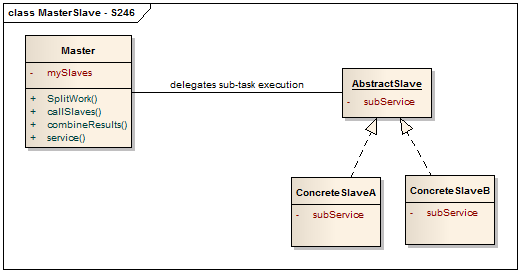
\includegraphics[width=0.7\textwidth]{content/posa1/images/master-slave-classes.png}
	\caption{Master-Slave Klassendiagramm}
\end{figure}


Die Slave-Komponente kann eine Unteraufgabe lösen welche vom Master gestellt wurde. Innerhalb der Master-Slave-Struktur gibt es mindestens zwei Instanzen von Slave-Komponenten welche mit dem Master verbunden sind.

\subsection*{Dynamics}

\begin{figure}[H]
	\centering
	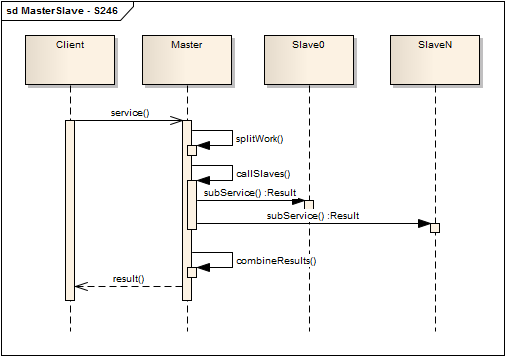
\includegraphics[width=0.7\textwidth]{content/posa1/images/master-slave-sequence.png}
	\caption{Master-Slave Sequenzdiagramm}
\end{figure}

\begin{enumerate}
	\item Ein Client fordert einen Dienst des Masters an.
	\item Der Master unterteilt die Aufgabe in mehrere Unteraufgaben.
	\item Der Master delegiert die Ausführung dieser Unteraufgaben an die Slave-Instanzen, startet ihre Ausführung und wartet auf die Ergebnisse.
	\item Die Slaves führen die Unteraufgabe aus und geben das Resultat ihrer Berechung an den Master zurück.
	\item Der Master berechnet ein Endergebnis für die ganze Aufgabe aus den Resultaten von den Slaves.
	\item Der Master gibt dieses Resultat zurück an den Client.
\end{enumerate}


\begin{enumerate}
	\item Unterteile die Arbeit in gleiche Subtasks. Anzahl der Subtasks kann (/sollte) der Nummer von zur Verfügung stehenden Prozessoren entsprechen.
\end{enumerate}

\begin{enumerate}
	\item Kombiniere die Resultate der Unteraufgaben.
\end{enumerate}

\begin{enumerate}
	\item Spezifiziere die Kooperation zwischen dem Master und den Slaves. Slaves müssen über die Aufgaben, die ihnen vom Master zugeteilt wurden informiert werden. Zum Beispiel als Argument beim Aufrufen des Subservices oder aus einem Pool von Subtasks.
	\item Implementiere die Slave-Komponenten gemäss der Spezifikations aus dem vorherigen Schritt.
	\item Implementiere die Master-Komponente gemäss der Spezifikation aus den Schritten 1 bis 3.
\end{enumerate}


:: Todo, evtl Erklärungen der einzelnen Varianten :::

\begin{itemize}
	\item Master-Slave für Fault-Tolerance: Die selbe Arbeit wird an eine fixe Anzahl Slaves verteilt. Sobald der erste Slave die Berechnung beendet hat, wird dessen Resultat an den Client zurückgegeben. n-1 Slaves können als ausfallen ohne die Berechnung zu verhindern. Um ein Fehler in einem Slave zu entdecken können z.B. Timeouts verwendet werden. Der Master bleibt jedoch Single Point of Failure.
	\item Master-Slave für Parallel-Computation: Die meistverbreitete Variante (siehe TSP Beispiel). Wichtig ist eine möglich gleichmässige Aufteilung der Arbeitslast zwischen den Slaves.
	\item Master-Slave für Computational Accuracy: Die Berechnung wird an mindestens 3 verschiedene Implementierungen delegiert. Das schlussendliche Resultat wird durch eine Wahlstrategie aus den Resultaten der Slaves berechnet:
	\begin{itemize}
		\item Nimm das Resultat, das von den meisten Slaves zurückgegeben wurde
		\item Nimm den Durchschnitt aller Resultate
		\item Antworte mit einem Fehler falls unterschiedliche Resultate empfangen wurden
	\end{itemize}
	\item Slaves as Processes
	\item Slaves as Threads
	\item Master-Slave mit Slave-Koordination: Notwendig falls der Zustand eines Slaves auf dem Zustand der anderen Slaves basiert. Entweder regeln die Slaves die Koordination direkt unter sich oder der Master übernimmt deren Koordination.
\end{itemize}

\subsection*{Known Uses}

\begin{itemize}
	\item Martizen Multiplikation (jede Reihe in der Produktmatrix kann individuell berechnet werden)
	\item Transformation eines Bildes
	\item Kreuzkorrelation von zwei Signalen
	\item Sortieren (z.B. Mergesort oder Quicksort)
\end{itemize}

\begin{itemize}
	\item Workpool model
	\item Gaggles
	\item Calibre DRC-MP
	\item CheckMate
	\item SPS ( Beckhof ) Master Leitrechner, Slave Feldmodule ( Umrechnen Teillogik)
	\item Akka: Scala / Java Toolkit für die Entwicklung von verteilten Systemen. Baut auf dem Actor Model auf in dem die Aktoren auch in Master/Slave Beziehungen zueinander stehen können.
\end{itemize}


\subsection*{Conequences}


\subsubsection*{Benefits}


\begin{itemize}
	\item Austauschbarkeit und Erweiterbarkeit
	\item Seperation of concerns
	\item Effizienz
\end{itemize}

\subsubsection*{Liabilities}


\begin{itemize}
	\item Umsetzbarkeit
	\item Machinenabhängikeit
\end{itemize}